% Metódy inžinierskej práce

\documentclass[10pt,twoside,english,a4paper]{article}

\usepackage[english]{babel}
\usepackage[T1]{fontenc}
\usepackage[IL2]{fontenc} % lepšia sadzba písmena Ľ než v T1
\usepackage[utf8]{inputenc}
\usepackage{graphicx}
\usepackage{url} % príkaz \url na formátovanie URL
\usepackage{hyperref} % odkazy v texte budú aktívne (pri niektorých triedach dokumentov spôsobuje posun textu)

\usepackage{cite}
\usepackage{times}
\usepackage{ragged2e}


\pagestyle{headings}

\title{Application of vector algebra and physics in designing steering behaviours of autonomous agents for realistic display in two dimensions\thanks{Semestrálny projekt v predmete Metódy inžinierskej práce, ak. rok 2022/23, vedenie: Mirwais Ahmadzai}} 

\author{Richard Čerňanský\\[2pt]
	{\small Slovenská technická univerzita v Bratislave}\\
	{\small Fakulta informatiky a informačných technológií}\\
	{\small \texttt{xcernansky@stuba.sk}}
	}

\date{\small November 3, 2022 } 

\begin{document}

\maketitle

\begin{abstract}

In this article we will focus on the problematic of steering behaviors of autonomous agents in software and display methods. The importance of this topic hides in usability in animation, film effects and mainly in games. If we want the user to have the best realistic experience from movement of the objects possible, we have to obey specific rules of physics that will be explained. Applying the knowledge, we will then see methods how to simulate a seek and arrival steering behavior. As a tool we will use a p5.js library of JavaScript language.

\end{abstract}

\section{Introduction}

Development in animation and games forces the creators to make the games more and more realistic. One of the most important aspects of realistic perception of a game is the movement of objects and the animation itself. Designing movement behaviors of these objects is then necessary. 

In this article, we will call the objects autonomous agents. More about them will be explained in part \ref{definition of a.a.}. After understanding the concept of autonomous agents, we will state a problem in part \ref{problem to solve}. In part \ref{seek and arrive} we will have a closer look at the problem and derive some formulas necessary for the simulation. Finally, we will simulate the steering behavior, stated as a problem in p. \ref{problem to solve} by writing the code in p5.js (in p. \ref{code}).

\section{Autonomous agents} \label{autonomous agents}

\subsection{Definition of autonomous agents} \label{definition of a.a.}

The autonomous agents generally refer to an entity that chooses how to act in its environment without any influence from a global plan or a leader. In games, these agents are not controlled by a player, but they are important part of the game because their action can significantly influence the flow of the game. For example, a villain who runs away from police decides on his own that he wants to escape and starts an action. There are three key components of autonomous agents we want to keep in mind \cite{Verhagen}. 

\begin{enumerate}
\item An autonomous agent has limited ability to perceive its environment. It makes sense that if autonomous agent must decide on its action, it should be somehow aware of the environment it is located in. The question here is how much limited the ability is. If we wanted the object to be all-knowing creature aware of everything else around it, we need to give it an access to information about everything. On the other side if we wanted it to have just very narrow view of the environment, let’s say just a few pixels around it.

\item An autonomous agent processes the information from its environment and calculates an action. The action is represented as a force that influences the object. For example, a police officer sees a thief and is attracted to him. The attraction is represented by a force pointing towards his location. 

\item An autonomous agent should have no leader. This is not something that defines every autonomous agent. Sometimes you need to state some global rules that it must follow, but mostly you want the object to decide on its own\footnote{however, the designer can include some specific atributes if needed}, calculate its own actions.

\end{enumerate}

\subsection{Types of behaviors according to the number of objects involved} \label{types of behaviors}

Craig Raynolds in his paper from Game Developers Conference \textbf{Steering Behaviors For Autonomous Characters} \cite{Raynolds} introduces some types of behaviors that could appear talking about autonomous agents and how they behave. They divide into two main groups:

\begin{itemize}
\item Simple behavior for individuals and pairs\newline
Containing only one or two autonomous agents.

\item Combined behaviors and groups\newline
Containing more than two autonomous agents.

\end{itemize}

In this article we will focus on the first mentioned. 

\section{Problem statement} \label{problem}

\subsection{Braitenberg vehicle} \label{braitenberg}

Braitenberg vehicle is an entity that is a hypothetical self-operating machine that can make decisions about how to behave in an environment based on its sense perception. Valentino Braitenberg explains his concept in the book \textbf{Vehicles} \cite{Braitenberg}. Here is an example of that type of vehicle from the book:

\bigbreak

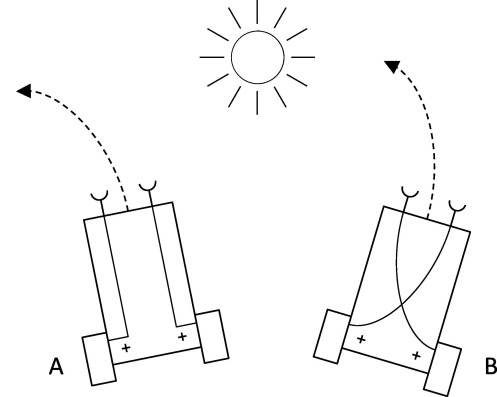
\includegraphics[scale=0.45]{braitenberg.jpg}
\quad Figure 1
\bigbreak
Vehicle A steers away from the light source and vehicle B steers towards the light source. It is not just about steering away or towards the sun. We could say that these vehicles feel emotion about the object. Vehicle A feels fear from the sun and vehicle B is attracted to it. We want the term vehicle to be clear because in the paper when we mention vehicle, we will be referring to the concept of Braitenberg vehicle and its characteristics. 

\subsection{Problem to solve} \label{problem to solve}

Let’s simulate a simple behavior for a pair (p. \ref{types of behaviors}). A vehicle (imagine a car) that wants to arrive to a specific position (f. e. parking lot). We could say that in the car there is a driver. He perceives the environment with his eyes and sees the location of the parking lot. Processes his distance from the place and calculates and action. He starts steering towards the parking lot (attraction towards the parking lot is the same as vehicle B in part \ref{braitenberg}). Notice the word steering here which is very important. We do not want to simulate an unrealistic car that is immediately able to turn around and head towards the target in a maximum speed. We want the animation to be smooth and realistically looking. What rules do we have to follow if we want to simulate a situation like this?


\section{Seek and arrive – a pursuit of a static target} \label{seek and arrive}

\subsection{Simple vehicle model} \label{model}
Craig Raynolds in his paper \cite{Raynolds} presents a simple vehicle model which I need to introduce to you. There are six attributes that our vehicle will have. 

Simple Vehicle Model: \{mass- scalar; position- vector; velocity-	vector; maxForce - scalar; maxSpeed- scalar; orientation- N basis vectors\}

\subsection{Characteristics of seek and arrive } \label{characterictics of seek and arrive}

\subsubsection{Seek} \label{seek}

Seeking steers a character towards a specified position in a space. This behavior aligns the vector of a velocity towards the target. But how do we calculate the steering force if we do not want the vehicle to steer completely right after seeing the target? We can diagram our problem from \ref{problem to solve}.

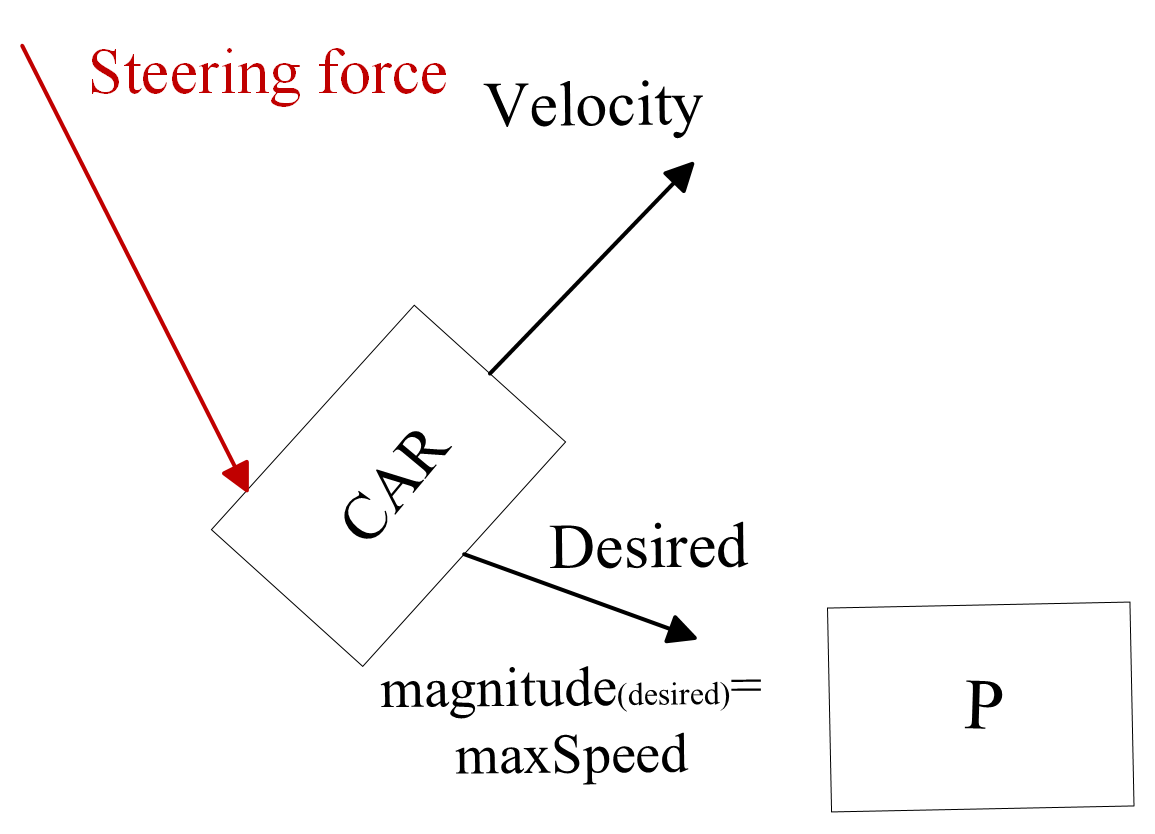
\includegraphics[scale=0.25]{diagram_car.png} 	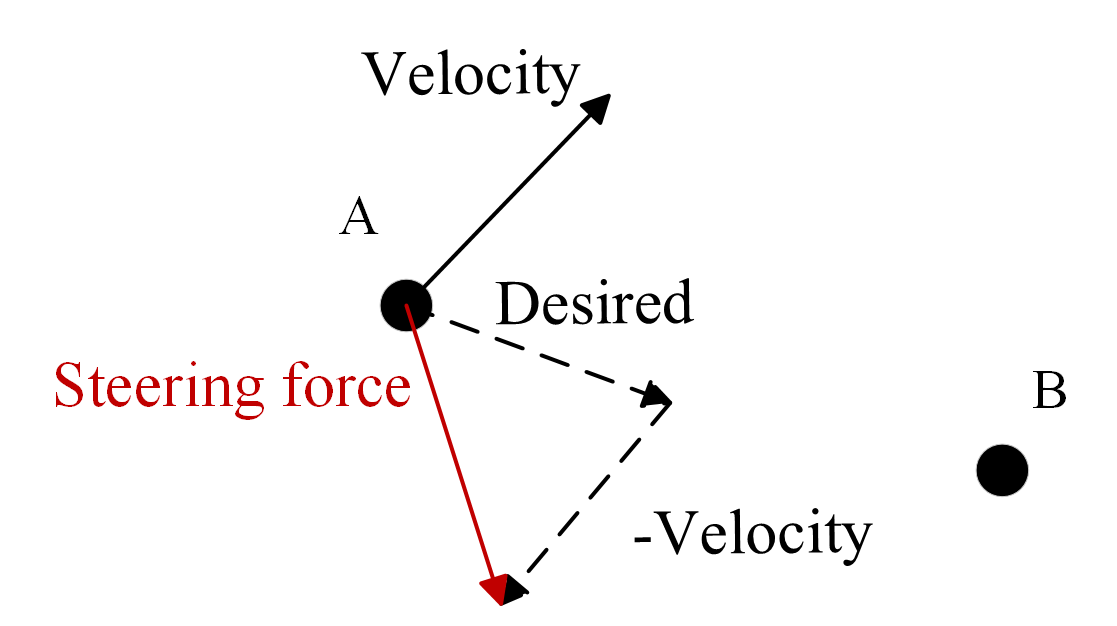
\includegraphics[scale=0.25]{diagram_steeringForce.png}\par
\quad Figure 2 
\hspace*{\fill} Figure 3
\bigbreak

The steering force is then calculated with this formula * as shown in the Figure 3.

\begin{center}
$desired =position A - position B \quad (vectors)$ \par
$ *steering force= desired – velocity$

\end{center}

\subsubsection{Arrive} \label{arrive}

When we want to simulate arrival, we must think about gradually decreasing the speed of the vehicle and eventually stop it. The following diagram describes the situation.

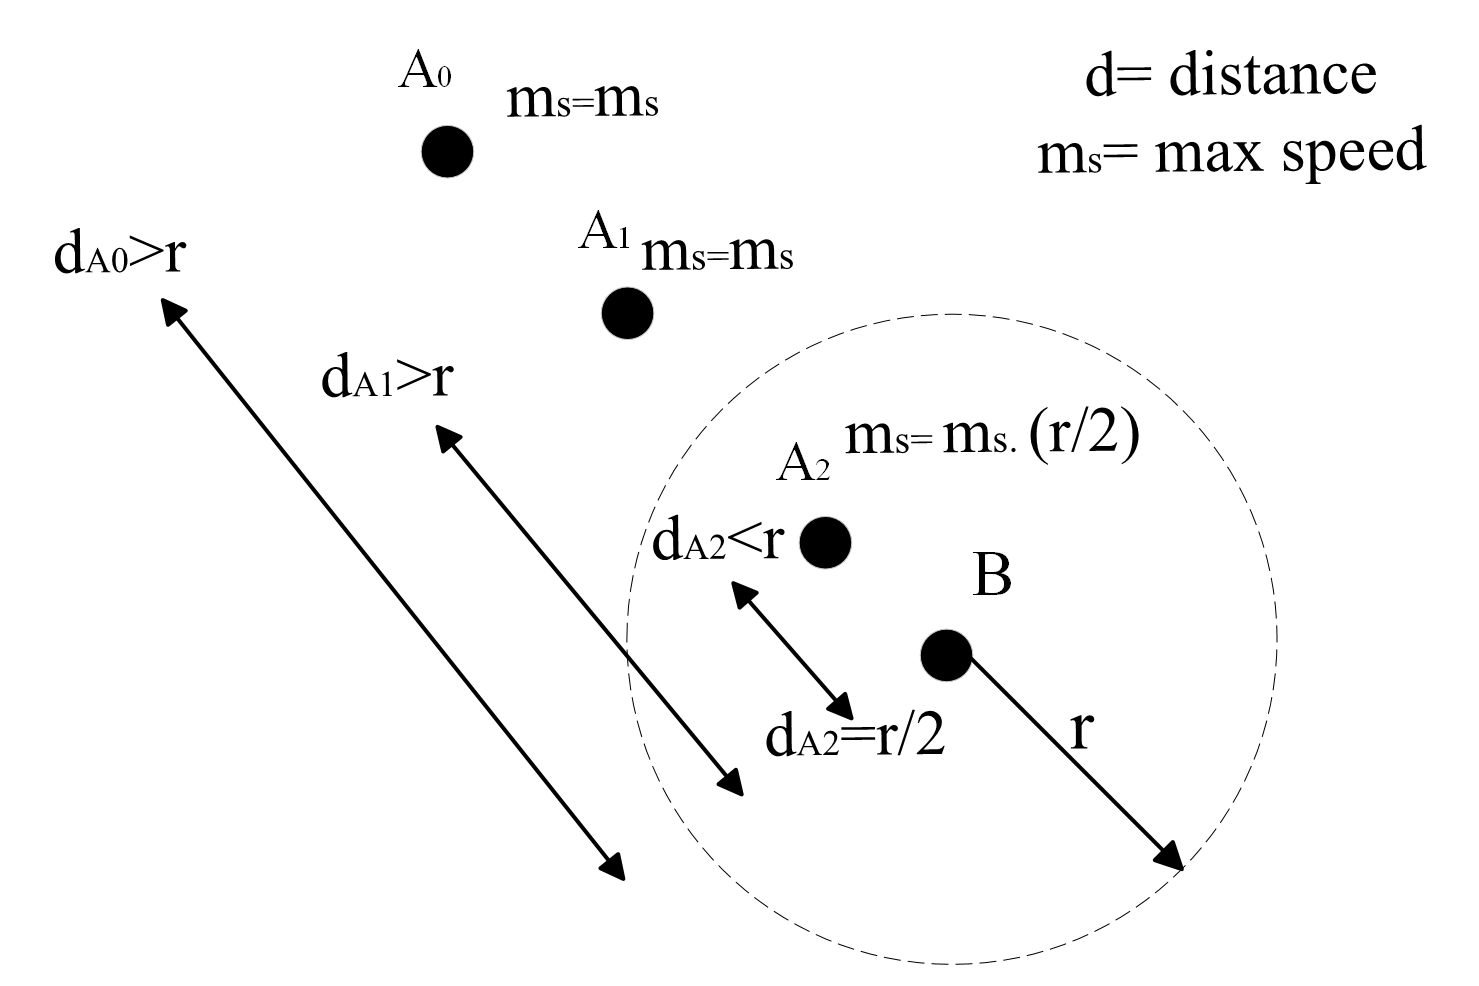
\includegraphics[scale=0.25]{diagram_radius.png}\par
Figure 4
\bigbreak


From the Figure 4 we can assume two things: 

\begin{center}

$d>r 	\Rightarrow speed = maxSpeed$ \par

$d \leq r \Rightarrow speed = (d/r)  . maxSpeed$

\end{center}		


\section{Simulating the behavior in p5.js} \label{simulation} 

\subsection{What is p5.js?} \label{p5 char} 

p5.js is a JavaScript library for creative coding, with a focus on making coding accessible and inclusive for artists, designers, or educators. It is a collection of pre-written code and provides us with tools that simplify the process of creating interactive visuals with code in the web browser. p5.js is free and open source. We will use it to simulate the problem. 

\subsection{Writing the code } \label{code} 

(Just a comment. Here I plan to explain certain parts of the code according to the explanation from part 4.2. The code is already done, and you can check it \textbf{\underline{\href{https://editor.p5js.org/RichardCernansky/sketches/E0zAXshWw}{here}}}... Clicking on the play button in the left corner runs the simulation.)

\subsubsection{class Vehicle} \label{class vehicle} 

\section{Other possible steering behaviors} \label{other} 

\section{Conclusion} \label{coclusion} 

\section*{Acknowledgement}
I would like to thank my friend Lukáš Častven for introducing the problem to me and arousing my interest in the topic\ldots

\bibliography{literatura}
\bibliographystyle{plain} 

\end{document}
